As though it was always destined to happen, your team has encountered
the time-traveling eccentric known only as Professor Whatsit. Well, not
so much ``encountered'' as ``collided'', as witnessed by the 
telephone-booth-shaped breach in your starboard hull.

This whacky master of time with a penchant for fezzes and bow ties promises to
repair your ship, but he first needs your help preventing a
Time Crash. You're not sure what that is exactly (he describes it as a
``timey-wimey, wibbly-wobbly sort of thing''), but as it seems to be 
related to a puzzle, you agree to pitch in.

It seems that the six groups of numbers listed on your
\textbf{Dimensional Barcodes} sheet coorespond to several dimensions
of space-time. To convert each group into a barcode, it seems that
the numbers should be written top-to-bottom in order from highest to lowest, 
and then these numbers should
be connected in order of how close they are, with the closest numbers
being connected first. The illustration below shows how the group
\texttt{06-21-65-79-91} can be barcoded.

As luck would have it, the so-called ``arc-word'' given by
these number groups is not only the key to preventing the Time Crash,
but it is also one of the secret codewords your team has been looking
for!

\begin{center}
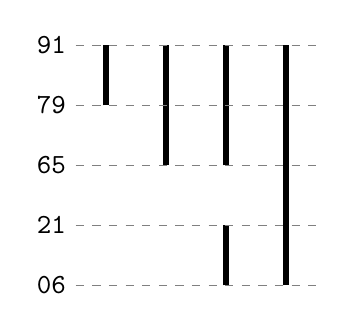
\begin{tikzpicture}[x=0.3in,y=0.3in] 
\fill[white] (0,0) rectangle (3,4);
\draw[line width=2pt] (0,3) -- (0,4); 
\draw[line width=2pt] (1,2) -- (1,4);
\draw[line width=2pt] (2,0) -- (2,1); \draw[line width=2pt] (2,2) -- (2,4); 
\draw[line width=2pt] (3,0) -- (3,4); 
\node[left] at (-0.5,0) {\tt06};
\node[left] at (-0.5,1) {\tt21};
\node[left] at (-0.5,2) {\tt65};
\node[left] at (-0.5,3) {\tt79};
\node[left] at (-0.5,4) {\tt91};
\foreach \y in {0,1,2,3,4} {
\draw[dashed,black!50] (-0.5,\y) -- (3.5,\y);
}
\end{tikzpicture}
\end{center} 
